\section{Footstep Evaluation Network}

The results of this model are very promising, with the model able to
predict footstep cost maps with high accuracy.
\autoref{fig:data-cn-typical-comparison}
shows the model output and ground truth for typical data sample.
\autoref{fig:data-cn-challenging-comparison}
shows a particularly challenging data sample, and the model is still
able to identify the best positions for each leg,
particularly the back left leg, which needs to be far from the
nominal position to maintain stability in that state.

\begin{figure}
  \centering
  \begin{minipage}[T]{0.45\textwidth}
    \centering
    \includegraphics[width=\textwidth]{images/data/training/typical-expected.png}
  \end{minipage}
  \hfill
  \begin{minipage}[T]{0.45\textwidth}
    \centering
    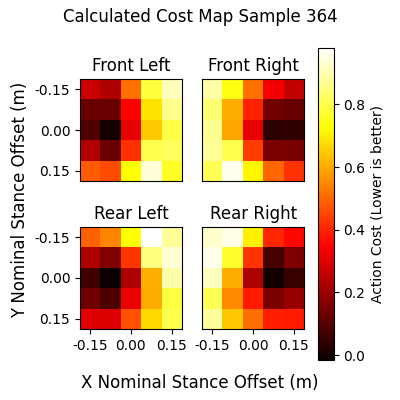
\includegraphics[width=\textwidth]{images/data/training/typical-calculated.png}
  \end{minipage}
  \hfill

  \caption{Typical data samples showing calculated (left) and
  expected (right) quadruped images.}
  \label{fig:data-cn-typical-comparison}
\end{figure}

\begin{figure}
  \centering
  \begin{minipage}[T]{0.45\textwidth}
    \centering
    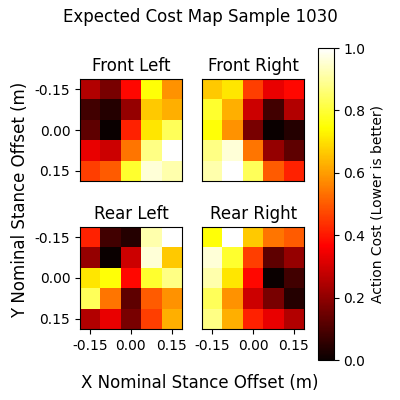
\includegraphics[width=\textwidth]{images/data/training/challenging-expected.png}
  \end{minipage}
  \hfill
  \begin{minipage}[T]{0.45\textwidth}
    \centering
    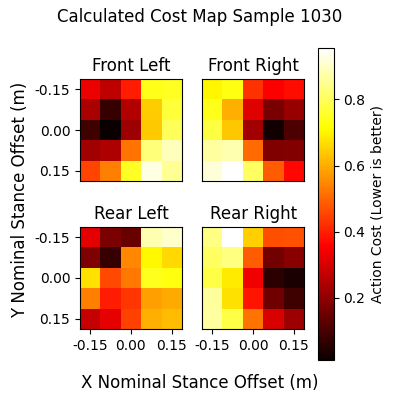
\includegraphics[width=\textwidth]{images/data/training/challenging-calculated.png}
  \end{minipage}
  \hfill

  \caption{Particularly challenging data samples showing calculated (left) and
  expected (right) quadruped images.}
  \label{fig:data-cn-challenging-comparison}
\end{figure}
